Die Ausgangsspannung wird \"uber zwei  Bananenstecker  $X_{6A}$ und $X_{6B}$ ans
\"Aussere    des    Geh\"auses     gef\"uhrt.     Die    Ausgangsspannung    ist
verpolungsgesch\"utzt mit der Diode $V_4$.

\begin{figure}[th!]
    \center
    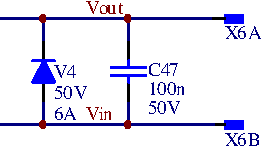
\includegraphics[width=.35\textwidth]{images/circuit/output-connectors.pdf}
    \caption{Verpolungsschutz am Ausgang}
    \label{fig:circuit:output}
\end{figure}

Damit die ADCs und DACs  m\"oglichst  genau messen und m\"oglichst in Full-Range
betrieben    werden   k\"onnen,   wird   eine   externe   Referenzspannung   von
\SI{1.5}{\volt}    verwendet     (siehe    Abbildung    \ref{fig:circuit:vref}).

\begin{figure}[th!]
    \center
    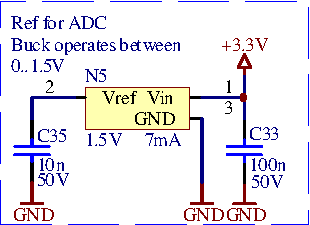
\includegraphics[width=.4\textwidth]{images/circuit/vref.pdf}
    \caption{1.5V Referenzspannung um die ADCs m\"oglichst in Full-Range betreiben zu k\"onnen}
    \label{fig:circuit:vref}
\end{figure}
